\chapter{信息论基础}\label{chap:information-theory}

信息是什么?不同于真实的物理世界,信息仿佛看不见,摸不着. 然而,任何人都可以体会到信息的存在,信息是我们认识世界的基础. 信息的存在正如同物理世界中的能量、动量一般,抽象而具有一般性. 信息论已经在计算机、AI、认知理论等诸多领域中得到了广泛的应用. 本章探讨信息论的基础,并给出他们在AI中的一些应用. 

在\Cref{sec:entropy},我们讨论熵的概念与性质. 在\Cref{sec:kl-divergence},我们讨论Kullback-Leibler散度的概念与性质. 在\Cref{sec:proofs},我们给出本章中的技术性较强的定理证明. 

\section{熵}\label{sec:entropy}


\subsection{概念的导出}

我们常说“恐惧来源于未知”,信息似乎代表着某种确定的东西,某种知识,因而和不确定性有相反的关系。更精确地说,\emph{消除不确定性的东西被称为信息.} 当然,这句话本身似乎是一种循环论证,它并没有真正回答信息或者不确定性到底是什么。所以我们进一步的问题是,给定一个“对象”,如何定量衡量它不确定性(或信息量)?

然而,单个对象的信息是一个非常难以划定的概念。同样的内容,对于不同的人来说,信息量是完全不同的。比如说,已经学过信息论的读者再看这一部分内容,他获得的信息一定比没有学过的读者要少得多。因而实际上,一种更加容易的办法是我们将世界视为不确定的,因而有多种可能的对象,然后考虑这一堆对象的信息量. 比如说,这本书的读者的背景是不确定的,可能学过信息论,也可能没学过,但是我们可以综合考虑不同读者的背景,然后给出一个信息的概率分析。

我们可以用数学来表述上面的考虑,假如我们进行一次试验,一共有$n$种可能的结果,第$i$种发生的概率为$p_i$. 我们预测试验的结果,如果越能正确地预测,那么就说明我们对这个试验中包含的信息知道的越多. 假如$p_1=1$,那么我们完全确定试验一定会产生结果$1$. 如果$p_i=1/n$,那么我们完全无法预计试验的结果. 我们对试验结果的预期与试验结果的概率分布有密切联系. 因此概率分布给我们带来了\textbf{信息}\index{信息},使得我们能够产生不同的判断. 另一方面,概率分布带来了\textbf{不确定性}\index{不确定性},使我们不能总是确信预言会成真. 

我们遵循“信息论之父”Shannon的思路,为信息提供一个严格的数学模型:熵。假设随机变量$X$表示了所有可能的结果(编号为$1$到$n$),$\Pr(X=i)=p_i$,$p=(p_1,\dots,p_n)$,有时候也把$p_i$写作$p(i)$. 我们把不确定性度量记为$H(p)$. Shannon假设$H$满足以下三个性质:
\begin{enumerate}
    \item $H$是一个连续函数.
    \item $n=1$时,$H(p)=0$。此外,事件结局可能数变多则不确定性增大:$p_i=1/n$时,$H(p)$随$n$单调递增.
    \item 如果一个试验被分成了两个相继的试验,那么原来的$H$应该等于分开之后的$H$的加权和.
\end{enumerate}

\begin{remark}
    第三个假设可以用下图来理解. 
\begin{center}
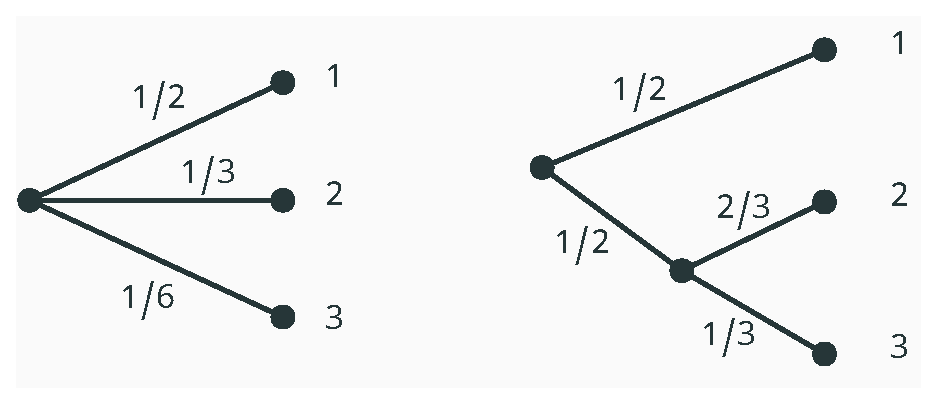
\includegraphics[width=0.4\textwidth]{Parts/information-and-data/decomposition-assumption.eps}
\end{center}

    假设我们有一个试验,有三种可能的结果,$1,2,3$,概率分别为$1/2,1/3,1/6$. 该试验的不确定性是$H(1/2,1/3,1/6)$. 我们把试验分成两步相继的试验,第一步试验有两种可能的结果,概率分别都是$1/2$。当第一步试验出现上面的结果时,第二步试验以概率$1$产生结果$1$;当第二步试验出现下面的结果时,第二步试验以概率$2/3$产生结果$2$,以概率$1/3$产生结果$3$. 我们可以看到,分成两步之后,第一步试验的不确定性是$H(1/2,1/2)$,第二步试验的不确定性有一半概率是$0$(上面的分支),有一半概率是$H(2/3,1/3)$(下面的分支),因而加权的不确定性是$1/2\cdot 0+1/2\cdot H(2/3,1/3)$. 因此第三个假设可以具体表述为
\[
H\left(\frac{1}{2},\frac{1}{3},\frac{1}{6}\right)=H\left(\frac{1}{2},\frac{1}{2}\right)+\left[\frac{1}{2}\cdot 0+\frac{1}{2}\cdot H\left(\frac{2}{3},\frac{1}{3}\right)\right].
\]
\end{remark}

这里,我们看Shannon的哲学思想:不确定性只来自于概率分布而不是具体对象。他的考虑具有浓厚的工程意味,正如他自己所说:“消息是具有含义的……然而,通信的语义层面并不是工程问题所关心的。“正是因为抽象掉了具体考虑的对象,信息论的应用才变得如此广泛。

基于上面三个假设,Shannon证明了如下定理,这一定理直接给出了熵的概念.

\begin{theorem}[Shannon定理]
    $H$满足三个假设当且仅当
    \[H(p)=-C\sum_{i}p_i\log p_i,\]
    其中$C$是正常数,$0\log 0=0$.\lhysays{留一个习题,说明这个定义的合理性}
\end{theorem}
根据对数的的换底公式,可以将$C\log p_i$写为$\log_bp_i$,这里$C=1/\log b$。于是,Shannon定理直接给出了熵的如下定义:
\begin{definition}[熵]
    分布列$p=(p_1,\dots,p_n)$的\textbf{熵}\index{熵}定义为
    \[H(p)=-\sum_{i=1}^np_i\log_b p_i.\]
    其中$b=2$或$\e$(自然对数底数),$0\log 0=0$.
\end{definition}

通常来说,使用$\e$作为底数会使得数学推导简洁,而用$2$为底数则常常是讨论信息量时的习惯。在后面通信理论中,我们将讨论熵在通信中的含义,以$2$为底的时候熵的实际意义会更清楚些。如果没有特别强调,我们在讨论时总是假设$b=\e$.

熵的定义还可以用数学期望的形式写出. 假设$X$的分布列是$p$,$p(i)=\Pr(X=i)$,那么我们也可以把熵写成期望的形式:
\[H(p)=-\E[\log p(X)].\]
每一个(离散)随机变量$X$会确定一个分布列$p_X$,因此我们也可以定义随机变量的熵:
\begin{definition}[随机变量的熵]
    随机变量$X$的\textbf{熵}\index{熵!随机变量的~}定义为
    \[H(X)=-\E[\log p_X(X)].\]
    其中$p_X$是$X$的分布列,$0\log 0=0$.
\end{definition}

尽管从信息论的角度我们可以唯一确定熵的定义,但是熵的概念在物理学上早就已经存在. 下面我们给出统计力学中熵的推导过程. 在经典力学中,物理系统的状态由粒子的位置和动量(速度)完全确定,将粒子位置和动量可能的值集合称为\emph{相空间},于是物理系统的演化就是相空间中的粒子状态的变化. 将相空间等分成$m$个单元,编号$1$到$m$. 假设相空间中有$N$个可区分的粒子,相互独立,没有相互作用,每个粒子等可能出现在每一个单元中. 如果单元$i$中有$N_i$个粒子,那么按照粒子在单元中的分布来看,系统处于某个特定状态的概率为
    \[P=\frac{N!}{N_1!\dots N_m!}\left(\frac1m\right)^N.\]
这是一个多项分布. 两边取对数,得
    \[\log P=\log(N!)-\sum_i\log(N_i!)-N\log m.\]
考虑充分大的$N_i$,由Stirling公式,有
\begin{align*}
    \log(N_i!)\sim\log\left(\sqrt{2\pi N_i}\left(\frac{N_i}{e}\right)^{N_i}\right)\sim N_i\log N_i.    
\end{align*}
因此,\lhysays{留作练习}
    \[\log P\sim N\log N-\sum_i N_i\log N_i- N\log m\sim N\log N-\sum_i N_i\log N_i.\]
假设$N_i$充分大的时候,$N_i/N$呈现固定的比例$p_i$,那么
    \begin{align*}
        N\log N-\sum_i N_i\log N_i&=N\log N-\sum_i Np_i\log(Np_i)\\
        &=-N\sum_i p_i\log p_i.
    \end{align*}
 $\log P\sim -N\sum_i p_i\log p_i$. 于是我们证明了:
    \[\frac1N\log P\to H(p_1,\dots,p_m),\quad N\to\infty.\]
因此,熵刻画了充分多粒子的物理系统某种特定状态出现概率!熵越大的系统越有可能达到. 更进一步,在统计力学中有Boltzmann $H$-定理:孤立的粒子系统会向着熵($H$)增加的方向演化,并最终达到熵最大的状态. $H$-定理是热力学第二定律的微观解释,熵越大的系统出现概率越大、越混乱、越接近均衡.

\subsection{概念与性质}
现在,我们将进一步探讨熵的若干拓展定义,并讨论他们的性质。

首先,我们考虑最简单的情形,即分布列为$(p_1,p_2)$,此时,我们不妨设$p_1=p$,$p_2=1-p$,那么熵就是
    \[H(p_1,p_2)=H(p)=-p\log p-(1-p)\log(1-p).\]
$H$是关于$p$的函数,作图如\Cref{fig:entropy-figure}所示.
\begin{figure}[ht]
        \centering
        \includegraphics[height=0.3\textheight]{Parts/information-and-data/entropy-figure.pdf}
        \caption{熵$H(p)$的图像.}
        \label{fig:entropy-figure}
\end{figure}

利用导数的方法,很容易证明,$H(p)$在$p\in (0,1/2)$严格单调递增,在$p\in (1/2,1)$严格单调递减. 它的最小值是$0$,在$p\in\{0,1\}$取得;它的最大值是$\log 2$,在$p=1/2$取得. 这与我们对于“不确定性”的直觉是相一致的:当$p$接近$0$或$1$时,我们对于$X$的取值几乎是确定的,因此熵接近$0$;当$p$接近$1/2$时,我们对于$X$的取值几乎是完全不确定的,因此熵接近最大值$\log 2$. 实际上,这样的性质对于一般的分布也是成立的.

考虑一般分布的熵$H(p)=H(p_1,\dots,p_n)$. 我们有如下性质:
\begin{proposition}\label{prop:entropy-nonnegative}
    $H(p)\geq 0$,等号成立当且仅当某个$p_i=1$.
\end{proposition}
\begin{proof}
这是一个典型的证明,主要的技巧是使用熵的期望形式。考虑随机变量$X$,其分布列为$p$. 回忆Jensen不等式:如果$f$是一个严格凸函数,那么
\[\E[f(X)]\geq f(\E[X]).\]
等号成立当且仅当$X$是常数.

因为$-\log(\cdot)$是严格凸函数,所以根据Jensen不等式
\[H(X)=\E[-\log p(X)]\geq-\log\E[p(X)]\geq -\log 1=0.\]
等号成立当且仅当$X$是常数,即对某个$i$,$p(i)=1$.
\end{proof}

\section{Kullback-Leibler散度}\label{sec:kl-divergence}

\begin{remark}
现代的主流信息论都是从Shannon发展起来的。然而,这一信息论也有很多问题。首先,信息论使用了概率论进行建模。然而我们已经看到,概率要么是作为频率的近似理论(频率学派),要么反映了人们对未知的信念(主观学派)。无论哪种解释,都将问题简化了。正如Kolmogorov所说:“如果事情没有按照我们的预期发展,那么问题一定出在我们对于概率和真实世界的随机之间关系不清晰的认识上。”其次,这一信息论考虑的是一族对象的信息。我们是否能够用这样的方式来衡量单个对象的信息量呢?比如,我们要考虑这本书中包含的信息量,是它放在所有可能的书的集合中去考虑呢,还是把它的每一个章节分开考虑成一个随机序列呢?因此,信息论并不能很好地回答“单个对象”的信息量的问题。

现代概率论的奠基人Kolmogorov也非常严肃地考虑了这一问题。他提出了被后世称为\textbf{Kolmogorov复杂度}\index{Kolmogorov复杂度}的概念,旨在刻画一个随机字符串的随机程度。简单来说,一个字符串的Kolmogorov复杂度就是描述它所需要的最短的代码长度,越随机的字符串就越需要更复杂的程序去描述它的产生方式。利用这一概念,我们可以将信息的概念变成一个对象自己的属性,而不再需要把对象放在可能的一堆对象中去考虑。这是信息论的另一种构建思路。
\end{remark}



\begin{appsec}
\section{附录:定理的证明}\label{sec:proofs}
\end{appsec}

\section{练习}

\section{章末注记}
信息一词的英文是“information”,从动词“inform”来,意思是告知、通知. 早在15世纪中叶,“information”一词的出现了义项“在通信中针对特定主题的知识”. 这说明在那个时候人类就已经意识到,通信会产生新的东西,被称为知识或信息. 然而,人类对信息的严谨探索起步晚得多. 关于信息的物理学讨论源自统计力学,Boltzmann提出了著名的熵,证明了H定理,这一定里在通信理论中揭露其更加深刻的本质. TODO